%tex2image density=3100, border=10

\documentclass[preview, border=2pt]{standalone}
\usepackage{amsmath}
\usepackage{amsfonts}
\usepackage{amssymb}
\usepackage{tikz,amsmath}
\usetikzlibrary{positioning,calc}
\begin{document}

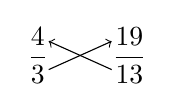
\begin{tikzpicture}[
    every node/.style={inner sep=0}
]
\node (frac1) {$\dfrac{4}{3}$} ;
\node[right=8mm of frac1] (frac2) {$\dfrac{19}{13}$} ;
\draw[->] ($(frac1.north east)!0.75!(frac1.south east)$)
            -- ($(frac2.north west)!0.25!(frac2.south west)$) ;
\draw[<-] ($(frac1.north east)!0.25!(frac1.south east)$)
            -- ($(frac2.north west)!0.75!(frac2.south west)$) ;
\end{tikzpicture}

\end{document}
